\documentclass[
	%a4paper, % Use A4 paper size
	letterpaper, % Use US letter paper size
]{jdf}

\addbibresource{references.bib}

\author{Bronson Lim}
\email{blim45@gatech.edu}
\title{Project 1 Report: Martingale}

\begin{document}
%\lsstyle

\maketitle


\begin{abstract}
	In this report, we investigate the pure Martingale betting system and the modified version where we have limited funds.
\end{abstract}

\section{Introduction}
In this investigation, we developed a simple gambling simulator that simulates the results of betting on the outcomes of
American roulette. We implemented two betting schemes:
\begin{enumerate}
	\item The unbounded Martingale scheme, see Experiment 1.
	\item The bounded Martingale scheme, see Experiment 2.
\end{enumerate}
We simulated the outcomes when repeatedly betting on black (47.4\% odds \cite{wiki:Roulette}); however, it is similar for red. The simulations consisted of
1000 consecutive bets which we call \textit{episodes}.

\section{Experiment 1}

In experiment 1, we simulated the outcomes over 10 episodes, where 1 episode was 1000 bets. If we reached \$80 in winnings, the simulation was ended and the remaining
spins were kept at \$80. The outcomes for the 10 episodes are in Figure \ref{fig:martingale_no_limits_simulation}. The mean plus/minus the standard deviation
are plotted in Figure \ref{fig:martingale_no_limits_mean} and the median plus/minus the standard deviation are plotted in Figure \ref{fig:martingale_no_limits_median}

\begin{jdffigure}
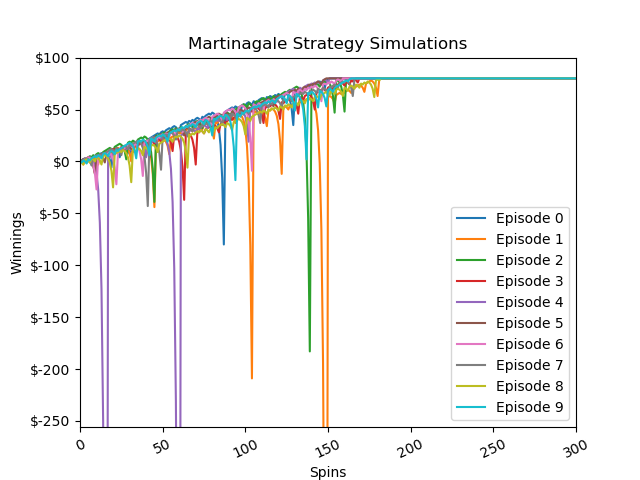
\includegraphics[height=8cm]{../../martingale/martingale_no_limits_simulation.png}
\captionof{figure}{Mean of the No Limits Martingale Simulation}\label{fig:martingale_no_limits_simulation}
\end{jdffigure}

\begin{jdffigure}
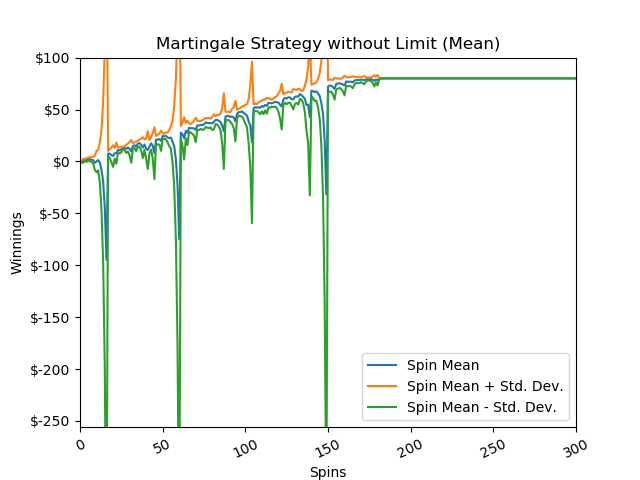
\includegraphics[height=8cm]{../../martingale/martingale_no_limits_mean.png}
\captionof{figure}{Mean of the No Limits Martingale Simulation}\label{fig:martingale_no_limits_mean}
\end{jdffigure}

\begin{jdffigure}
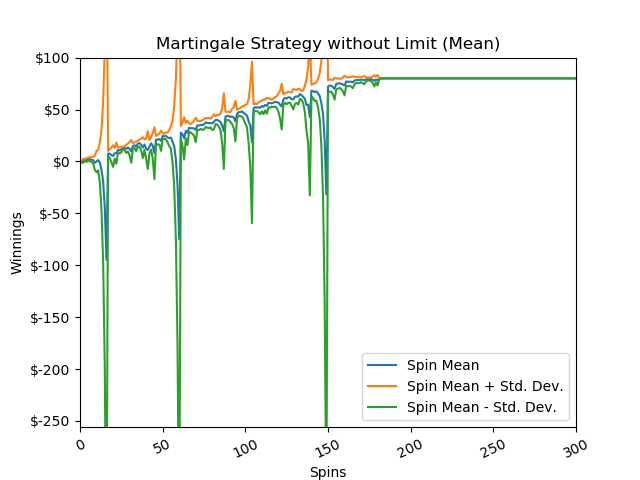
\includegraphics[height=8cm]{../../martingale/martingale_no_limits_mean.png}
\captionof{figure}{Mean of the No Limits Martingale Simulation}\label{fig:martingale_no_limits_median}
\end{jdffigure}

\section{Experiment 2}
In Experiment 2, we imposed the condition that we cannot lose more than \$256. In this martingale scenario with a limited bankroll, we again plotted the mean and median
plus/minus the standard deviation for a series of 10 episodes. The mean is in Figure \ref{fig:martingale_with_limits_mean} and the median is in Figure
\ref{fig:martingale_with_limits_median}.
\begin{jdffigure}
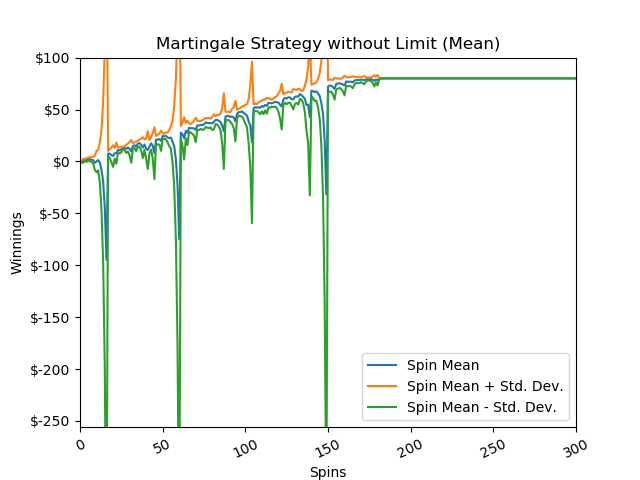
\includegraphics[height=8cm]{../../martingale/martingale_no_limits_mean.png}
\captionof{figure}{Mean of the No Limits Martingale Simulation}\label{fig:martingale_with_limits_mean}
\end{jdffigure}

\begin{jdffigure}
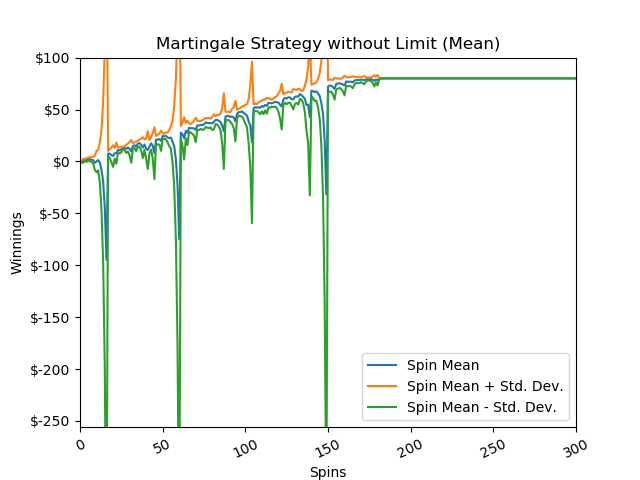
\includegraphics[height=8cm]{../../martingale/martingale_no_limits_mean.png}
\captionof{figure}{Mean of the No Limits Martingale Simulation}\label{fig:martingale_with_limits_median}
\end{jdffigure}

\section{Analysis}

\subsection{Question 1}
The probability of winning \$80 in 1000 sequential bets using the martingale double down strategy with a reset amount of \$1 is 1, at least experimentally. More mathematically,
the probability of winning is 47.4\%. Every time we win, we have a net positive of \$1 which can be easily computed by analyzing the value of
\(2^n-2^{n-1}-\cdots-2-1\). So we really are just asking if it's possible to win 80 times within 1000 spins. Hence, this is just a binomial distribution problem
and we are computing the probability of at least 80 successes in 1000 trials. This is very close to 1.

\subsection{Question 2}
The expected value is \$80 after placing 1000 sequential bets. This is because the probability of reaching \%80 is very close to 1. Once we reach \$80 in winnings
our strategy is to stop playing. Since we are essentially assured the win, the expected value is \$80.

\subsection{Question 3}
The upper and lower standard deviation lines are discrete and finite so they must reach a maximum/minimum. This means the real question is: do they converge, and therefore stabilize?
Yes, they converge. Again, we are almost surely expected to win by 1000 spins. The data supports that it will be far sooner than that for each episode.
Once all episodes win \$80, the standard deviation is zero so the upper and lower standard deviation lines converge to the mean/median.

\subsection{Question 4}
In Experiment 2, 7 of the 10 episodes reached \$80 winnings. Therefore experimentally, the probability of winning is 0.7. Although, I would prefer to do more careful
analysis with a larger sample size.

\subsection{Question 5}
The data from Experiment 2, indicates there are essentially only two outcomes: win \$80 or lose \$256. Therefore we will assume the probability of
our bankroll sitting between these amounts is negligible. Let \(X\) represent winnings, then \(X\) takes two values and the expected value, \cite{wiki:ExpectedValue}, is computed as:
\[
	E[X] = p(X=80)\cdot \$80 + p(X=-256)\cdot(-\$256) =\$-20.80.
\]


\subsection{Question 6}
Again, the data is discrete and finite so the upper and lower standard deviation line must reach a maximum/minimum value.
They do in fact stabilize as our data supports that you either quickly get to \$80 in winnings or quickly lose all of your \$256 bankroll.
Once all 10 episodes have reached their outcome, the standard deviation will become constant and therefore the upper/lower standard deviation lines
must stabilize.

\subsection{Question 7}
A sample size of 1 is never good. We could have, by chance, observed an outcome which suggests our strategy was guaranteed to win or to lose.
Instead, using Monte Carlo simulations to compute expected values gives us a more rigorous expectation of the outcome of our strategy. That is, one benefit
is expected values give us a more realistic idea of what we should expect in the long run. We can then make informed decisions and alter our strategy, in this case,
to attempt to raise the expected value.

\section{References}
\printbibliography[heading=none]


\end{document}
